\section{Framework structure}
\label{sec:framework}
In order to assess Atlas' aptitude as a interference measurement platform, we
continue by presenting our framework which is based on Atlas.

\subsection{RIPE Atlas background}
% Some basic information about Atlas.
Founded in 2010 by RIPE NCC, Atlas~\cite{atlas} is a globally
distributed Internet measurement network consisting of physical probes hosted
by volunteers.  Once a user connects her probe to the network, it can be used
by other participants for measurements. So-called \emph{credits} are awarded
automatically based on the uptime of contributed probes, which are expended in
order to perform custom measurements. Queries to probes can be initialized
centrally either over the web frontend, or over a RESTful API.

% Geographic and topological distribution.
An ideal measurement platform features high geographic and
topological diversity, thereby facilitating measurements in any region where
filtering occurs.  While Atlas probes are distributed throughout the world,
there is a significant bias towards the U.S. and Europe as can be seen in
Figure~\ref{fig:probe_distribution}.  As for Atlas' topography, only 68
autonomous systems contain 40\% of all Atlas probes with the three most common
autonomous system numbers being 7922 (4.4\%, Comcast Cable Communications),
3320 (3.2\%, Deutsche Telekom), and 6830 (2.8\%, Liberty Global Operations).
While not optimal, most censoring regions still contain at least several
probes.

\begin{figure}[t]
\centering
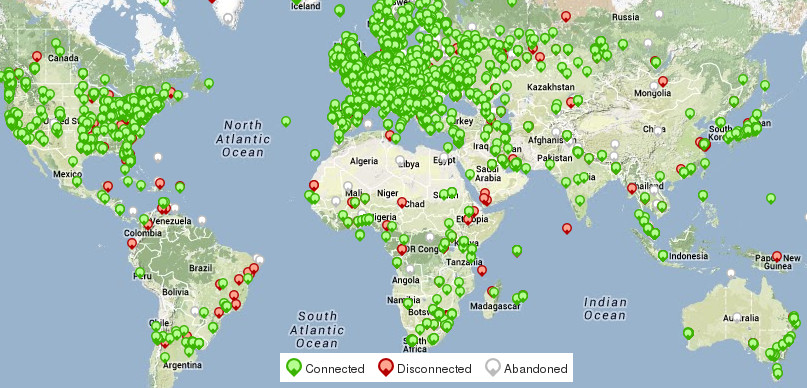
\includegraphics[width=0.48\textwidth]{diagrams/probe_distribution.jpg}
\caption{The geographic distribution of Atlas probes as of May 2014.  Green
icons represent active probes whereas red icons represent probes which are
currently offline.  The distribution is heavily biased towards the U.S. and
Europe.} \label{fig:probe_distribution}
\end{figure}

% What kind of measurements does Atlas allow?
As of May 2014, Atlas allows four types of measurements; ping, traceroute, DNS
resolution, and X.509 certificate fetching (henceforth called SSLCert).  All
four measurement types can further be parameterized for more fine-grained
control.  HTTP requests are not possible at this point due to abuse and
security concerns.  While Atlas clearly lacks the flexibility of comparable
platforms (see Table~\ref{tab:comparison}), it makes up for it with high
diversity, responsiveness, and continued growth.  After all, we do not expect
Atlas to replace existing platforms, such as OONI, but rather to
\emph{complement} them.

% We also need to mention how you can stablish a big experiments using RIPE.
% And mention about the propblem of how you frist need to submit your
% experiments and then it will give you predicted cost. This way we can move to
% cost function.

\subsection{Atlas cost model}

As briefly mentioned above, Atlas measurements have to be paid with special
credits.  The exact ``price'' of a measurement depends on the measurement type,
its parameters, and the destinations.  The credit system works based on a
linear cost model.  Each user has a credit balance that can be increased
steadily by hosting Atlas probes or by receiving credits from other users.

Table~\ref{tab:cost} lists the currently available measurement types as well as
their associated costs.  While DNS and SSLCert measurements have a fixed cost,
ping and traceroutes vary depending on the amount and sizes of packets.  Also,
one-off measurements cost twice as much as repeated measurements.  When
scheduling a new experiment, the user first specifies the details (e.g.,
measurement type as well as measurement parameters).  Afterwards, Atlas'
web-based frontend calculates the measurement costs on the server side and
shows it to the user.  Finally, upon completion of the measurement, the
respective cost is subtracted from the user's credit balance.

Due do the non-deterministic nature of pings and traceroutes, and measurements
in general, we developed a command-line based tool to help users create new
measurements and estimate their costs.\footnote{The tool is available at
\url{http://cartography.nymity.ch}.}  As input, the tool expects \emph{1)}
a country of interest, \emph{2)} the amount of credits, the user is willing
to ``pay'', and \emph{3)} a measurement type.  Our tool then determines the
amount of available probes (if any), the expected costs, and runs the
measurement if the cost is below the user's expected cost.

%\subsection{Calculating Costs}
%
%Predicted cost = $\sum_{i=1}^{5} (C_i * N_i)$  where i can be (DNS, SSL, ...)\\
%Remaining credits = min(available cost, desired cost) - predicted cost
%
%Note that it is a linear cost model so number of probs included doesn't matter
%in the cost part it matters when we suggest the experiment by just uniformly
%distribute the possible number of measurements on one(total experiments
%possible/Num probs)
%This should be included in the API philipp wrote (TODO)
%
%one-off measurements cost twice as much as not one-off.

% \subsection{Evaluation of our cost model}
% To test that our cost prediction is accurate, we ran a series of unit cost with
% different values, and compared  the suggested cost and the actual credit
% subtracted with the cost our approach suggest. Because the number of possible
% cases are finite we can run all unit measurements, then calculate confidence
% interval to show how good we do.
% 
% We choose a prob(12214) 

\begin{table}[t]
\centering
\begin{tabular}{lc}
\textbf{Measurement} & \textbf{Cost in credits} \\
\hline 
DNS\slash DNS6 (TCP) & 20\\ 
DNS\slash DNS6 (UDP) & 10\\ 
SSLCert\slash SSLCert6 & 10 \\
Ping\slash Ping6 & $N * (int(S/1500)+1)$\\
Traceroute\slash Traceroute6 & $ 10*N*(int(S/1500)+1)$\\[1ex] 
\hline 
\end{tabular} 
\caption{The cost for all available Atlas measurements.  The variable $N$
refers to the number of packets whereas the variable $S$ refers to packet
sizes.}
\label{tab:cost} 
\end{table}

<<<<<<< HEAD
\subsection{Considerations in Assessing Measurement Validity}

Despite their distribution across a diversity of countries and networks, RIPE Atlas may not fully reflect the Internet as it is experienced by the general public, as probes neither fully emulate the network position nor the configuration of an average user. As an immediate control, efforts are taken to verify the reachability of non-controversial content and identify whether probes use domestic name servers. These probes may be excluded from measurements in order to avoid Type 1 and Type 2 errors.

Even with additional precautions, incongruences across observations are an inevitable a product of the high rate of placement of probes on commercial and academic networks. These institutions may have alternative connectivity that is faster and less highly regulated than consumer networks. Additionally, disrupting or degrading connections based on plaintext data, traffic classification or application headers would fall outside of the measurements currently possible with Atlas probes. Lastly, Atlas, as with most measurements outlined within Section~\ref{related_work}, is unlikely to detect content restrictions imposed by the platforms themselves, such as search result manipulation or withholding of content based on a user's physical location.

\subsection{Consensus Building}

The international distribution of web services, for purposes of performance, failover and load balancing, has created additional complexity in the determining whether answers received over the Internet are genuine. While SSL and DNSSEC utilize third-party trust to validate answers, Certificate Authorities have been previously compromised by state and non-state actors, and DNSSEC is not widely implemented. In order to validate answers within the Atlas network, we use a cross-country comparision of responses to queries. This methodology assumes that states that interfere with connectivity do not coordinate strategies internationally. States and Internet service providers impose different approaches to content-filtering for purposes of localization, infrastructure or even the monetization of blocked traffic. Furthermore, surveillance is more effective when the public is unaware of the practices and technologies employed against them, placing an strong incentive on secrecy and narrow targeting. Therefore, as a simple test of validity, we count the number of countries or ASNs that an answer, such as a DNS A record, final network of transit or a certificate hash, is seen. Any response with fewer than the mean number of jurisdictions or those within private network spaces (RFC 1918~\cite{rfc1918}) are treated a potentially aberrant and flagged for further investigation.

\subsection{Ethical Aspects}

Atlas was not designed as interference analysis platform and accordingly, its
=======
\subsection{Ethical aspects}
% The problem.
Atlas was not designed as censorship analysis platform and accordingly, its
>>>>>>> FETCH_HEAD
volunteers likely do not expect that their probes will be used for such
purposes.  Careless measurements could attract a censor's attention and cause
repercussions for probe operators.  In addition, an increased used of Atlas for
politically-sensitive analysis could scare away probe operators and jeopardize the
usefulness of the platform. These concerns extend beyond merely complying with Atlas's
acceptable usage policies and guide our selection of measurements.

Atlas' measurement types are limited to ping, traceroute, DNS requests and
X.509 certificate fetching.  As of May 2014, it is not possible to create HTTP
requests or engage in actual, meaningful communication with arbitrary
<<<<<<< HEAD
destinations, which limits the damage caused by reckless measurement. We are not aware of environments where network queries to commonly frequented platforms or services solicit attention from authorities, even when blocked, nor where answers are falsified in order to mitigate research. Requests for sites such as Facebook are generated as a part of normal web use due to script inclusion and Google Public DNS is commonly used due to its reliability. Highly trafficked sites are a different subset of potential monitoring candidates than content promoting child abuse or violent extremism. 
=======
destinations, which limits the damage caused by reckless measurement.
Nevertheless, we stress that great care must be taken when planning
measurements because the volume of measurements could still be suspicious.  We
believe that Atlas has a place in the domain of censorship analysis but it
has to remain a small place lest it endangers users or the platform itself.
>>>>>>> FETCH_HEAD

The balance between research interests and exposure to risk is an area of concern shared across all initiatives identified in Section~\ref{related_work}. This has stimulated a broader discussion that will play a factor in future utilization of Atlas. Nevertheless, we stress that great care must be taken when planning measurements because the volume and types of measurements could still be suspicious. For a more comprehensive ethical discussion, refer to Wright et al.~\cite[\S~5]{Wright2011}.
